\documentclass{article}
\usepackage[utf8]{inputenc}
\usepackage{graphicx,amsmath,subcaption}

\title{Physcis 20.3 Numerical Solutions of Ordinary Differential Equations}
\author{Sophie Li}
\date{February 2019}

\begin{document}

\maketitle

\section{The Motion of a Mass on a Spring}
Figure \ref{fig:expliciteuler} shows a few cycles of oscillation when the explicit Euler method is implemented. This graph was made with initial condition set to $h=0.004, N=10000, x_0=2, y_0=2, t_0=0$.
\begin{figure}[h]
    \centering
    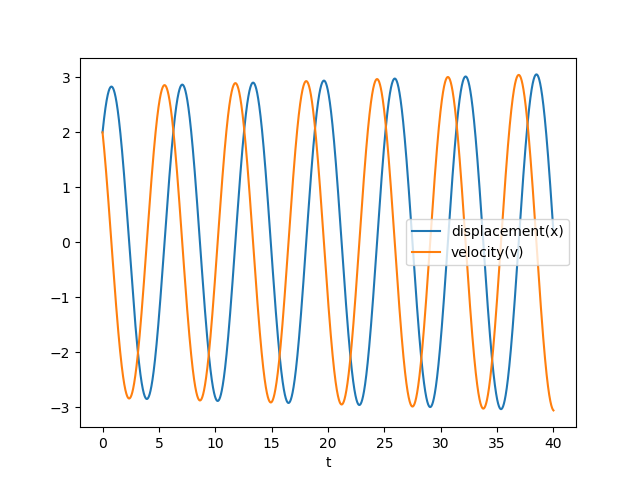
\includegraphics[width = \textwidth]{Images/expliciteuler.png}
    \caption{Motion of a mass on a spring implementing the explicit Euler method}
    \label{fig:expliciteuler}
\end{figure}

\section{Analytic Solution}
\subsection{Derivation of the Analytic Solution}
Rearranging $F=ma=-kx$ we have that $a=-\frac{k}{m}x$. Let $a=\frac{d^2x}{dt^2}$ and $\frac{k}{m}=\omega^2$. We then have $a=\frac{d^2x}{dt^2}=\omega^2x$. Using the Ansatz principle we guess that the solution to this equation is in its most general form $$x(t)=A\cos{\phi}\cos{\omega t}-A\sin{\phi}\sin{\omega t}$$.
This can be rewritten in terms of two new constants $B$ and $C$.
$$x(t)=B\cos{\omega t}+C\sin{\omega t}$$.
By finding the derivative of the above equation we get that 
$$v(t)=-B\omega\sin{\omega t}+C\omega\cos{\omega t}$$
To find the constants $C$ and $D$, substitute $t=0$ into both of the equations. 
$$v_0=v(0)=-\omega\sin{0}+C\omega\cos{0}=\omega C$$
So, $C=\frac{v_0}{\omega}$
$$x_0=x(0)=B\cos{0}+C\sin{0}=B$$
So, $B=x_0$
Therefore we have the general solution
$$x(t)=x_0\cos{\omega t}+\frac{v_0}{\omega}\sin{\omega t}$$
$$v(t)=-x_0\omega\sin{\omega t}+v_0\cos{\omega t}$$
But because $\omega = 1$ in this case we have that the final analytical solution to the mass of the spring is
\begin{equation}
    x(t)=x_0\cos{t}+v_0\sin{t}
\end{equation}
\begin{equation}
    v(t)=-x_0\sin{t}+v_0\cos{t}
\end{equation}
\subsection{Global Errors}
Figure \ref{fig:globalerrorexp} shows that as the global error increases exponentially with time. This graph was made with initial conditions set to $h=0.005, N=50000, x_0=2, y_0=2, t_0=0$. The increasing error could have also been seen at a lower $N$, however, a larger $N$ was chosen tot demonstrate the exponential increase.
\begin{figure}[h]
    \centering
    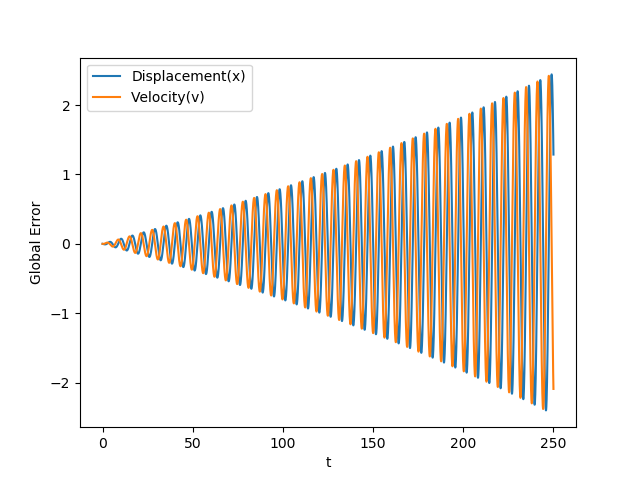
\includegraphics[width = \textwidth]{Images/globalerrorexp.png}
    \caption{Global errors between the analytic solution and the explicit Euler method}
    \label{fig:globalerrorexp}
\end{figure}

\section{Truncation Error}
Figure \ref{fig:truncerror} shows that the truncation error is proportional to $h$ for small values of h. We can see that as h increases, so does the truncation error. I chose $h_0=0.001$ and then calculated the error for $h_0,h_0/2,h_0/4,h_0/8,h_1/16$ to produce this plot. 
\begin{figure}[h]
    \centering
    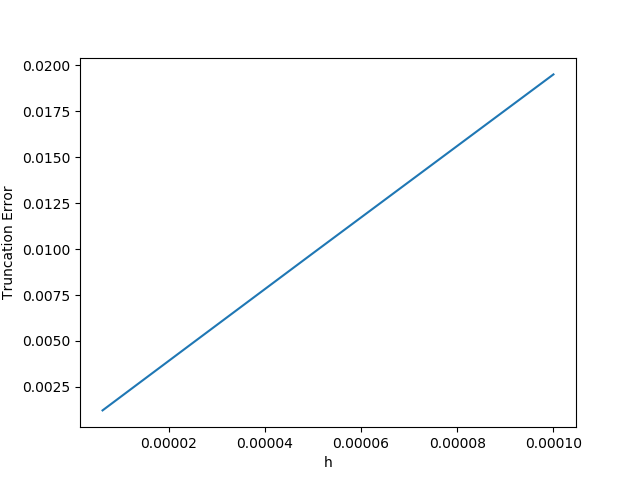
\includegraphics[width = \textwidth]{Images/truncerror.png}
    \caption{Maximum value of $x_{analytic}-x$ versus $h$ for several different $h$}
    \label{fig:truncerror}
\end{figure}

\section{Numerical Evolution of Total Energy}
One can calculate the normalized total energy of a physical system by $E=x^2+ v^2$. Figure \ref{fig:totalenergy} shows how this energy evolves over a long period of time. The trend we can see is that the energy increases exponentially with time. We can see that this is similar to the global error which we also saw to be increasing over time, see figure \ref{fig:globalerrorexp}. For this physical system we would actually expect the energy to remain constant as energy should be conserved. However, it is evident that due to the exponentially increasing error, E also increases exponentially. The parameters used for the plot of figure \ref{fig:totalenergy} are $h=0.004, N=100000, x_0=2, y_0=2, t_0=0$.
\begin{figure}[h]
    \centering
    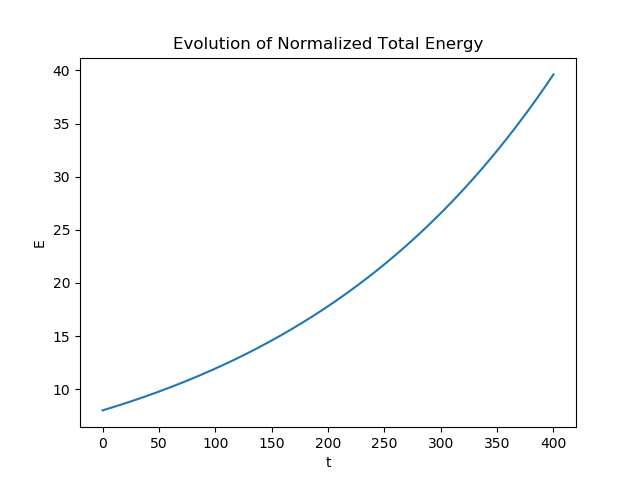
\includegraphics[width = \textwidth]{Images/totalenergy.png}
    \caption{Long term evolution of the total energy with time, explicit Euler method}
    \label{fig:totalenergy}
\end{figure}

\section{The Implicit Euler Equation}
\subsection{Expressions for the Implicit Euler Method}
The implicit Euler method requires the unknown values of $x_{i+1}$ to update the known values of $x_i$. This can be encoded in the linear system
\begin{equation}
\begin{pmatrix}
1&-h\\
h&1
\end{pmatrix}
\cdot
\begin{pmatrix}
x_{i+1}\\
v_{i+1}
\end{pmatrix}
=
\begin{pmatrix}
x_i\\
v_i
\end{pmatrix}
\end{equation}
However, we want to find an expression for the unknown $x_{i+1}$ in terms of the known value $x_i$. To do this we must first find the inverse of the first matrix. This gives
\begin{equation}
\begin{pmatrix}
1&-h\\
h&1
\end{pmatrix}
^{-1}
= \frac{1}{1+h^2}\cdot
\begin{pmatrix}
1&h\\
-h&1
\end{pmatrix}
=
\begin{pmatrix}
\frac{1}{1+h^2}&\frac{h}{1+h^2}\\
\frac{-h}{1+h^2}&\frac{1}{1+h^2}
\end{pmatrix}
\end{equation}
We can then use this inverse matrix to find the values of $x_{i+1}$ and $v_{i+1}$ in terms of $x_i$ and $v_i$. We get the linear system
\begin{equation}
\begin{pmatrix}
\frac{1}{1+h^2}&\frac{h}{1+h^2}\\
\frac{-h}{1+h^2}&\frac{1}{1+h^2}
\end{pmatrix}
\cdot
\begin{pmatrix}
x_i\\
v_i
\end{pmatrix}
=
\begin{pmatrix}
x_{i+1}\\
v_{i+1}
\end{pmatrix}
\label{linsys2}
\end{equation}
Using equation \ref{linsys2} we can get the implicit Euler method in terms of $x_i$ and $v_i$
\begin{equation}
    x_{i+1}=\frac{x_i}{1+h^2}+\frac{v_i}{1+h^2}, v_{i+1}=\frac{v_i}{1+h^2}-\frac{x_i}{1+h^2}
\end{equation}
If we plot these expressions much we get a graph like in figure \ref{fig:impliciteuler}. This plot looks extremely similar to the plot generated when implementing the explicit Euler equations. We can compare it to figure \ref{fig:expliciteuler} because the parameters used are exactly the same. 
\begin{figure}[h]
    \centering
    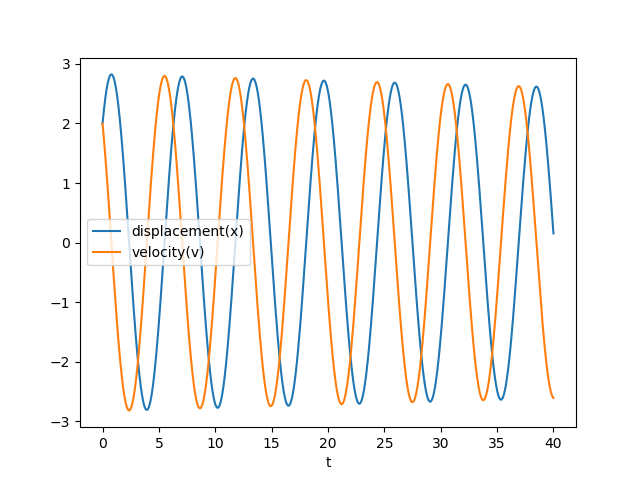
\includegraphics[width = \textwidth]{Images/impliciteuler.png}
    \caption{Implementing the implicit Euler equation}
    \label{fig:impliciteuler}
\end{figure}
\subsection{Global Errors}
If we plot the global errors generated using the implicit functions we get a graph like in fig \ref{fig:globalerrorimp}. This graph shows an evolution of total energy similar to figure \ref{fig:globalerrorexp} for the explicit Euler equation. However, the error does not exponentially increase like in figure \ref{fig:globalerrorexp}, instead it first increases and then tails off in a logarithmic fashion. Again, the graphs are comparable because I used the same parameters as for the explicit method.
\begin{figure}[h]
    \centering
    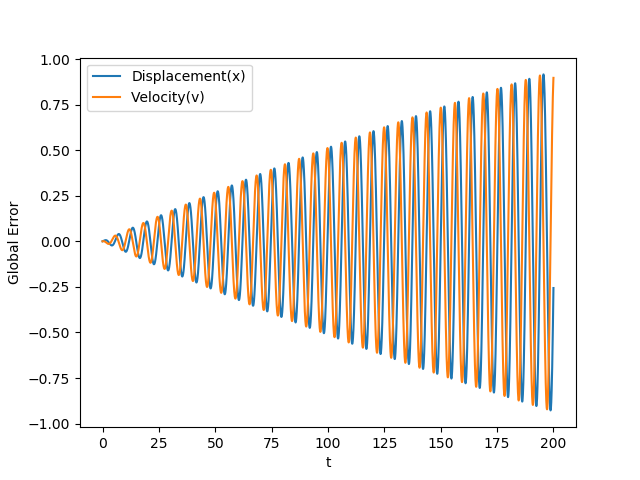
\includegraphics[width = \textwidth]{Images/globalerrorimp.png}
    \caption{Global errors between the analytic solution and the implicit Euler method}
    \label{fig:globalerrorimp}
\end{figure}
\subsection{Evolution of Total Energy}
Unlike in figure \ref{fig:totalenergy} for the explicit Euler equation, where the energy grew exponentially, the energy in figure \ref{fig:totalenergyimp} decreases exponentially. Again, the energy is not constant. Thus, the implicit Euler method also does not model the physical system such that energy is conserved. We saw that the error instead of increasing exponentially only had a logarithmic increase. It is because of this that we see a decrease in energy and the errors become greater for the implicit Euler method.
\begin{figure}[h]
    \centering
    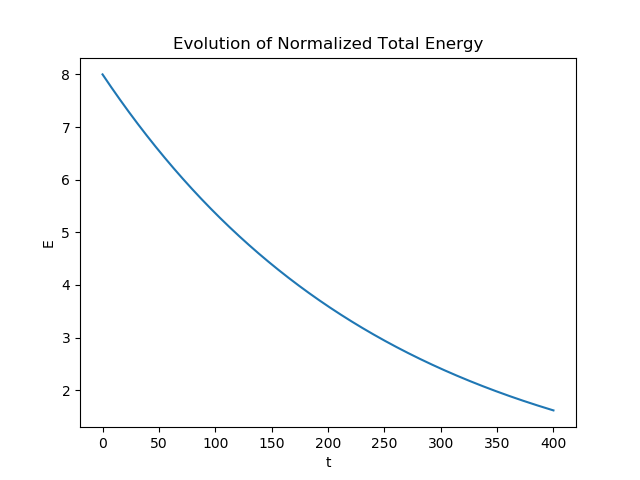
\includegraphics[width = \textwidth]{Images/totalenergyimp.png}
    \caption{Long term evolution of the total energy with time, implicit Euler method}
    \label{fig:totalenergyimp}
\end{figure}

\section{Phase-space Trajectories}
Figure \ref{fig:phase} shows very clearly that the errors in the explicit method deviate positively and the errors in the implicit method deviate negatively. We can see this because in the explicit Euler phase-space the deviation from the analytic solutions are towards the outside of the circle. This means that there are always positive errors calculated by this solution. On the other hand, for the implicit Euler method, the deviations are inside the orange circle and therefore, the errors were always negative.  
\begin{figure}[h]
    \centering
    \begin{subfigure}{0.7\textwidth}
    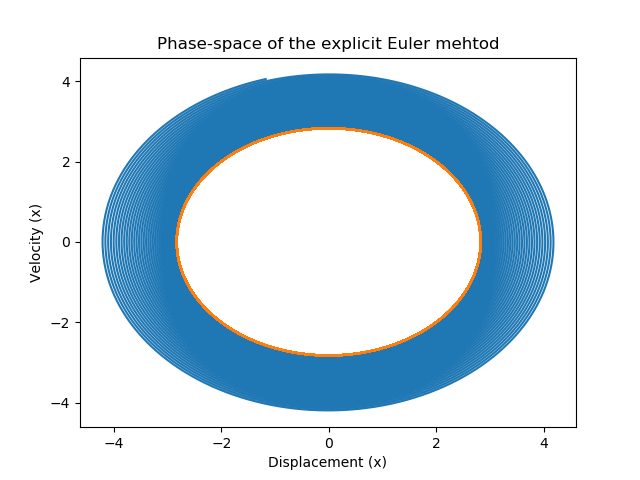
\includegraphics[width =\textwidth]{Images/phaseexp.png}
    \caption{Phase-space trajectory produces by the explicit Euler method}
    \end{subfigure}
    \begin{subfigure}{0.7\textwidth}
    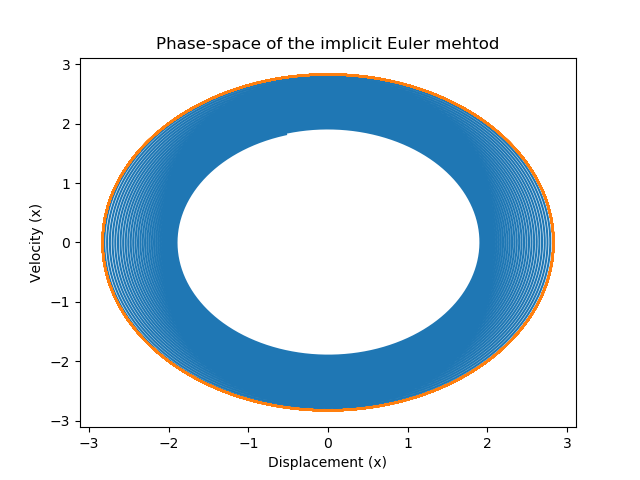
\includegraphics[width =\textwidth]{Images/phaseimp.png}
    \caption{Phase-space trajectory produces by the implicit Euler method}
    \end{subfigure}
    \caption{Phase-space trajectories produced by the implicit and explicit Euler methods. The orange circle in both represents the trajectory produced by the analytic solutions}
    \label{fig:phase}
\end{figure}

\section{Symplectic Euler Method}
\subsection{Phase-space trajectory}
When the phase space for the symplectic method is plotted along side the analytic for the value of $h=0.004$ that was also used in figure \ref{fig:phase}, we can see no difference between the analytic solutions and the solutions generated by the symplectic method. However, if the value of $h$ is decreased to $h=0.04$ we have figure \ref{fig:phasesymp}(b). The circle of the symplectic method slightly deviates from the analytic solutions, however, it corrects itself and returns back. Thus, it never diverges in one particular direction from the orange circle like in figure \ref{fig:phase}. 
\begin{figure}[h]
    \begin{subfigure}{0.5\textwidth}
    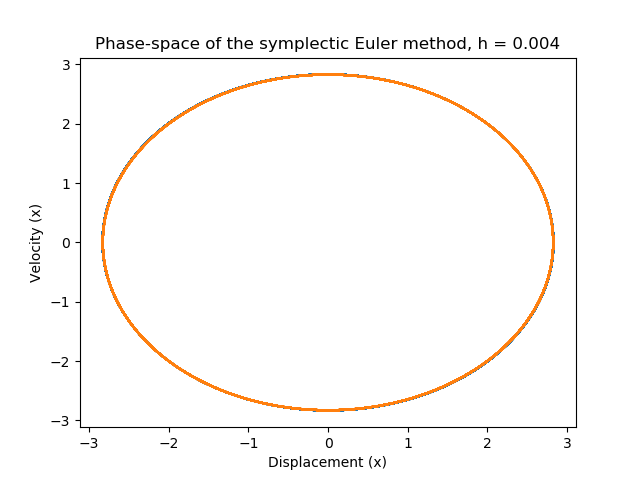
\includegraphics[width =\textwidth]{Images/phasesymp.png}
    \caption{Phase-space trajectory produced by the symplectic method at $h=0.004$}
    \end{subfigure}
    \begin{subfigure}{0.5\textwidth}
    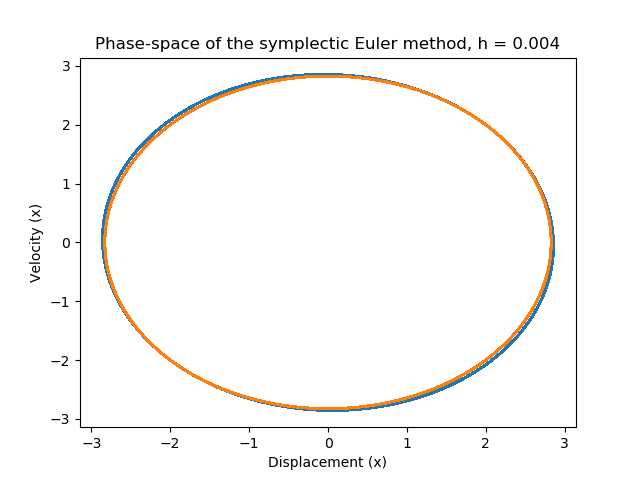
\includegraphics[width =\textwidth]{Images/phasesymplarge.png}
    \caption{Phase-space trajectory produced by the symplectic method at $h=0.04$}
    \end{subfigure}
    \caption{Phase-space trajectories produced by the symplectic Euler method at different values of $h$. The orange circle in both represents the trajectory produced by the analytic solutions}
    \label{fig:phasesymp}
\end{figure}
\subsection{Evolution of total energy}
Figure \ref{fig:totalenergysym} shows the long term evolution of the total energy of the symplectic Euler method compared to the analytical total energy. The analytic energy holds a constant value as expected because energy is conserved in the physical system. We can see that the energy of the symplectic grows, however when it reaches a certain height it returns to the total energy for the analytic solution. This suggests that the error of the symplectic method is in a sense, self-correcting. Although it does not fully conserve energy, it returns back to a given point. And therefore it never diverges significantly like in the explicit or implicit Euler methods. We can also relate figure \ref{fig:totalenergysym} to \ref{fig:phasesymp}(b). The way the energy error is corrected back is similar to the way that the symplectic trajectory deviated yet returned to the trajectory of the analytic solution. This suggests that the error created by the symplectic method is both positive and negative and thus self-correcting. 
\begin{figure}[h]
    \centering
    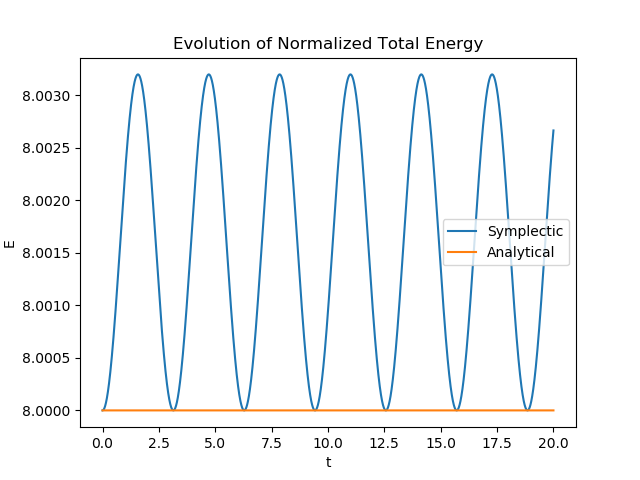
\includegraphics[width = \textwidth]{Images/totalenenergysym.png}
    \caption{Long term evolution of the total energy with time, symplectic Euler method}
    \label{fig:totalenergysym}
\end{figure}
\end{document}